\chapter{Trabalhos Relacionados}
\label{ch:TrabalhosRelacionados}

\section{sEMG e AM}
Como observado na revisão acadêmica de \cite{yousefi2014characterizing}, os estudos relacionados a sEMG e AM são separados em  dois tipos de transtornos neuromusculares miopatia e neuropatia, onde miopatia refere-se a um grupo de patologias que atingem diretamente o tecido muscular sem relação com disfunções do sistema nervoso. Já a neuropatia, onde encontra-se a doença de Parkinson, é caracterizada por qualquer dano nos nervos envolvidos no controle muscular. Ambos os casos possuem diferenças e similaridades, em resumo segundo \cite{yousefi2014characterizing} as diversas técnicas de AM sobre sEMG, pode-se catalogá-las em três etapas, análise, decomposição e classificação, sendo que não é necessariamente sequencial, podendo ser um processo iterativo.

Outro estudo com bons resultados, porém sem relação direta com a DP, foi desenvolvido por \cite{katsis2006novel}, que propôs um método para detectar automaticamente um PAUM e classifica-lo em normal, neuropático ou miopático. O método possui três etapas, pré-processamento do sinal EMG, detecção e agrupamento do PAUM, e posteriormente a classificação deste utilizando um SVM. Como resultados foi obtido foi possível identificar corretamente para o agrupamento 93, 95 e 92\% respectivamente, e para a classificação do PAUM foi alcançado aproximadamente 86\%. 

\subsection{Análise}
O pré-processamento ou análise dos dados é uma das partes mais importantes do processo de AM. Essa etapa ocorre apos a coleta dos dados, possuindo alguns objetivos como organizar os dados em conjuntos, identificar possíveis problemas como ruídos ou valores desconhecidos. Assim como, é comum utilizar esta etapa para simplesmente aprender mais sobre os modelos, plotando gráficos e colhendo mais informações. Também utiliza-se essa etapa para realizar tratamento nos dados, como transformações lineares para um conjunto de dados mais simples de ser trabalhado \cite{batista2003pre}. 

\subsection{Decomposição}
Segundo \citeonline{yousefi2014characterizing} a decomposição de um sinal EMG consiste de cinco etapas, aquisição, segmentação, extração de \textit{features}, agrupamento de MUPs e atribuição de MUP.

A seleção das \textit{features} ou características, é a distinção de um sinal bruto em informações úteis, esta informação tratada consiste uma \textit{feature}, a qual será utilizada para treinar o modelo, além disto busca-se remover a parte indesejada do sinal e interferências associadas \cite{phinyomark2012feature}.

Segundo \citeonline{phinyomark2012feature}, essa etapa deve ser trabalhada cuidadosamente, uma vez que erros podem prejudicar a classificação dos dados. Em sua pesquisa sobre as \textit{features} em EMG, verificou-se utilizando gráficos de dispersão, analise estatística e classificação, que a maioria das \textit{features} no domínio do tempo são redundantes e desnecessárias, sendo melhor agrupadas em quatro tipos: energia e complexidade, frequência, modelo de previsão e dependência do tempo. O estudo recomendou o uso das seguintes \textit{features}:

\begin{itemize}
    \item MAV: método de informação de energia;
    \item WL: informação de complexidade;
    \item WAMP: informação de frequência;
    \item AR: método de predição;
    \item MAVS: depedência  do tempo.
\end{itemize}

Outro estudo que cita algumas \textit{features} compiladas de outros trabalhos, Como observado na Figura \ref{featuresEMG} na página \pageref{featuresEMG}, de acordo com \citeonline{yousefi2014characterizing} as \textit{features} são as seguintes:

\begin{itemize}
    \item \textbf{Amplitude pico a pico}: relaciona os valores nas extremidades minima e máxima de ativação de uma MUP;
    \item \textbf{Tempo de ativação}: descreve a duração entre inicio e termino de ativação de uma MUP;
    \item \textbf{Área de uma MUP}: é obtida integrando á área do sinal gerado, resultante da duração do movimento de uma MUP;
    \item \textbf{Espessura}: é a razão entre a área e a Amplitude.
\end{itemize}

No trabalho realizado por \citeonline{yousefi2014characterizing}, um bom resultado foi obtido na decomposição, onde realizou-se uma classificação utilizando o algoritimo SVM, o qual obteve uma acurácia de 70.4\% no modelo, utilizando uma técnica de redução de dimensionalidade para a extração das \textit{feature}, a DWT (sigla do ingês: \textit{discrete wavelet transform }, transformada discreta de \textit{Wavelets}). Este método utiliza uma função capaz de remodelar uma função qualquer no domínio do tempo, em diferentes escalas de frequência e tempo, após a utilização desta técnica o algoritimo SVM obteve uma acurácia de 99.3\%.

Com relação a redução de dimensionalidade, no estudo desenvolvido por \citeonline{guler2005classification}, realizou-se uma uma classificação utilizando SVM e EMG, para a redução de dimensionalidade utilizou-se a combinação entre a FFT (sigla do inglês: \textit{fast Fourier transform}, Transformada rápida de Fourier), combinada com a PCA (Análise de Componentes Principais, sigla do ingês: \textit{Principal Component Analysis}). Esta combinação é para facilitar o calculo e armazenamento dos dados do sinal EMG. Por fim, \citeonline{guler2005classification} concluiu que o SVM possui uma alto nível de predição com relação aos sinais EMG.

\begin{figure}[h]
    \centering
     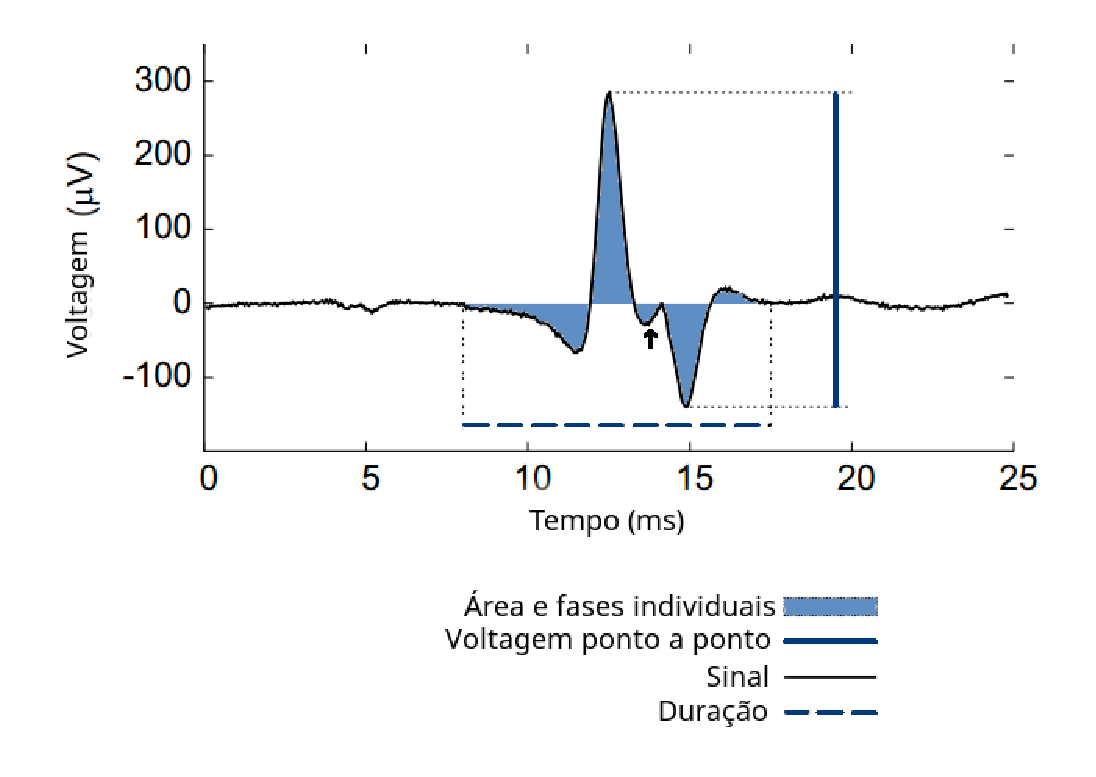
\includegraphics[width=1\textwidth]{figuras/featuresEMG.eps}
     \caption{\textit{Features} de um sEMG, adaptado de \citeonline{yousefi2014characterizing}.}
     \label{featuresEMG}
 \end{figure}

Outro trabalho com foco no estudo relacionado a eficiência dos métodos de redução de dimensionalidade, foi realizado por \citeonline{camara2015resting} que utilizou uma rede neural artificial para identificar a doença através do Tremor em repouso, \citeonline{ai2011classification} utilizou sEMG com SVM para identificar a doença de Parkinson e o Tremor essencial. Ele utilizou como técnica de redução de dimensionalidade, uma EMD (sigla do inglês: \textit{empirical mode decomposition}, decomposição em modo empírico) para decompor o sinal em IMF (sigla do inglês: \textit{intrinsic mode functions}, funções do modo intrínseco). E seguindo, decompôs as IMF em SVD (sigla do inglês: \textit{singular value decomposition}, decomposição em valores singulares) para extrair as \textit{features} das IMF geradas, com estre tratamento os dados são melhores calculados e processados pelo algoritimo SVM. Outro método de redução de dimensionalidade, foi aplicado por \citeonline{ai2011classification}, onde comparou-se o desempenho substituindo a EMD pela DWT e verificou através de validação cruzada que o método EMD-SVD foi superior ao método DWT-SVD.

\section{sEMG, AM e DP}
SVM também foi utilizada por \cite{kugler2013automated}, que combinou sEMG com sinais de um acelerômetro, para identificar a doença de Parkinson e o Tremor essencial, neste trabalho utilizou-se a validação cruzada, para verificar a integridade dos resultados.

Outro trabalho interessante foi realizado por \cite{loconsole2018model}, que propôs uma técnica em 3 estágios para diferenciar portadores da DP, foi utilizada uma analise caligráfica com sEMG, para a classificação dos dados, foi utilizado um SVM alinhada com uma rede neural artificial.

Com relação as \textit{features}, um comparativo sobre as estratégias de redução de dimensionalidade em EMG foi realizado por \cite{liu2014feature}, obtendo uma média de 95\% de precisão na classificação em com 12 \textit{features} selecionadas. 